\chapter{OpenHAB}

After analyzing the main products and services in the field of home automation and voice assistance, I must choose the solution
that can best fit this project. One of its requirements is to use as many open source and free technologies as possible, and that
the final product is easily usable by the final user and sufficiently flexible to adapt it to our needs.

OpenHAB is fully open source and completely free, and has reached a level of maturity where it is highly stable and intuitive. In its
most recent version, it provides an user interface that automatize many tasks that a standard user might not know how to do. And,
of course, it can integrate many devices from different vendors, as In have mentioned in the previous chapters, which is also one of
the most important matters for reaching our objective.

In this chapter, I will explore in depth this home automation platform and all its possibilities, in order to have a better general idea
about it when building the final system.

\section{Introduction}
As I mentioned in previous chapters, openHAB (open Home Automation Bus) is a completely free, technology agnostic and open
source platform for home automation. 

OpenHAB software is capable of integrating different domotic systems, devices and technologies into a single solution. It also
provides uniform user interfaces, and a common approach to automation rules across the entire system, regardless of the number
of manufacturers and sub-systems involved.\cite{openHABDocs}

The platform runs on many popular platforms including Linux, Windows and macOS. It is also popular to install it in systems like the
Raspberry Pi, and openHAB even provides a special distribution for this computer, called \textit{openHABian}, a simplified way of
getting up and running openHAB, but offering the complete experience.

OpenHAB defines also a community of users, contributors and maintainers, working together on the improvement of the system.
Everything related to the community is in the openHAB community forum. The community is very active and helpful, and thanks
to them I have always found a way to solve my issues.

\bigskip
\section{History of openHAB}
The history of openHAB begins in 2010, when Kai Kreuzer, a smart home enthusiast from Germany, developed in Java and using the
OSGi technology (Open Services Gateway Initiative) as the basis, which is a set of specifications that define a dynamic component 
system for Java. The use of this technology makes it easier to update the services independently and their implementation. It favor
the expandability of the system.

In 2013, openHAB becomes an official Eclipse project under the name of Eclipse SmartHome, but they decide to keep both projects
active and to develop them at the same time. In Eclipse SmartHome would maintain the architecture and the functionalities from the
previous openHAB, and in openHAB they would study how to integrate the different devices and technologies that it supports via 
add-ons.

The newest version, OpenHAB 2, has been the biggest change that OpenHAB has suffered since its initial launch. It includes more 
add-ons and some changes that simplify much more the process for developers, as well as implementing Apache Karaf underneath, 
which greatly extends its possibilities. In addition, the UIs have been improved, improving greatly the user experience. OpenHAB 2 is
much easier to install, and it automates many repetitive processes that might result hard for some users.

\bigskip
\section{Structure}
OpenHAB works thanks to add-ons, which can extend its capabilities to fit each user’s needs, from User Interfaces, to the ability to 
interact with a large and growing number of physical \textit{Things}. Add-ons may come from the OpenHAB 2 distribution, the Eclipse
SmartHome project Extensions, or from the OpenHAB 1 distribution.

\begin{figure}
	\centering
	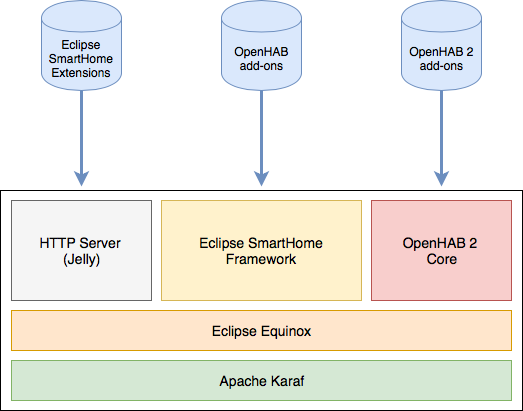
\includegraphics[width=0.9\textwidth]{images/Chapter_05/openhab-architecture.png}
	\caption{OpenHAB architecture}
	\label{fig:openhab-architecture}
\end{figure}

The figure \ref{fig:openhab-architecture} shows the overall architecture of openHAB 2. In the lowest layer, we can find Apache Karaf.
Apache Karaf is basically a modular and open source OSGi runtime environment that can host any kind of applications.\cite{apacheKaraf}
 
Next, there is Eclipse Equinox, which is also an implementation of the OSGi core framework specification. But the goal of the Equinox
project is to be a first class OSGi community and foster the vision of Eclipse as a landscape of bundles too. Equinox is responsible for
developing and delivering the OSGi framework implementation used for all of Eclipse.\cite{eclipseEquinox} 

The next and last level is divided in three parts. The first one is the Jetty HTTP server, also part of Eclipse, which provides a Web server 
and javax.servlet container, plus support for HTTP/2, WebSocket, OSGi, JMX, JNDI and JAAS, among others.\cite{eclipseJetty} Secondly,
we can find the Eclipse SmartHome Framework , the framework to build end user solutions on top like openHAB, that I mentioned 
before.\cite{eclipseSmartHomeDocs} The last part is the core of openHAB 2, which provides the full solution.

As the diagram in the figure \ref{fig:openhab-architecture} indicates, we can add to this system extensions from Eclipse SmartHome and
add-ons from the first and second version of openHAB.

\bigskip
\section{Concepts}
As Eclipse SmartHome is the logic part of OpenHAB 2, all the elements I am listing are part of it. Eclipse SmartHome strictly differentiates
between the physical view and the functional view of the system. The physical view is more familiar to us, and focuses on the devices
on the system, the connections between them (e.g. wires, Netatmo devices, WiFi hardware) and other physical aspects of the system.
The functional view focuses on how information about the devices, connections, and so on, is represented in user interfaces, focusing
on how rules effect representations of physical devices in software. The functional view focuses on how an action in a user interface
affects the software associated with the physical device it represents.\cite{openHABDocs}

That said, I will explore the different elements that Eclipse SmartHome considers in this section. The greatest difference that we can find
related to devices, is between \textit{Things} and \textit{Items}. Generally speaking, Things represent physical systems that can be added
to openHAB and Items represent functionalities that can be used by the applications. The figure \ref{fig:openhab-concepts-basics} 
shows a graphical explanation of this concept, though I will explain in depth these concepts below.

\begin{figure}
	\centering
	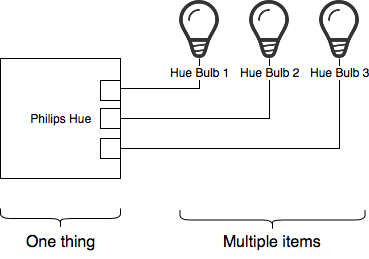
\includegraphics[width=0.6\textwidth]{images/Chapter_05/openhab-concepts-basics.png}
	\caption{A simplification of the concepts of Thing and Item}
	\label{fig:openhab-concepts-basics}
\end{figure}

\subsection{Things}
Things are the entities that can physically be added to a system and which can potentially provide many functionalities in one. They do
not need to be devices, but they can also represent a web service, or any other manageable source of information and functionality.
Things are important in the setup and configuration process, when the user has to add his devices to the system, but they are not for
the operation, when everything is up and running.

Things can have configuration properties, which can be optional or mandatory. Such properties can be basic information like an IP address,
an access token for a web service or a device specific configuration that alters its behavior.

\subsubsection{Channels}
Channels are part of the Things, and they represent the different functions they provide. Where the Thing is the physical entity 
or source of information, the Channel is a concrete function from this Thing. For example, some Philips Hue light bulbs have a color 
temperature Channel and a color Channel, both providing functionality of the one light bulb Thing to the system. For sources of
information the Thing might be the local weather with information from a web service with different Channels like temperature, pressure 
and humidity.

Channels are linked to Items, where such links are the glue between the virtual and the physical layer. Once such a link is established,
a Thing reacts on events sent for an item that is linked to one of its Channels. Likewise, it actively sends out events for Items linked to its 
Channels

\subsubsection{Bridges}
Bridges are special types of Things. They are \textit{Things} that need to be added to the system in order to gain access to other Things.
For example, an IP gateway for some non-IP based home automation system or a web service configuration with authentication information
which every Thing from this web service might need.

Some Bindings come with a Bridge, like the \textit{PHC Binding}, which allows to integrate modules of PHC in openHAB.\cite{openHABPHCBinding}

\subsubsection{Thing Status}
Every Thing has a status, which helps to identify possible problems with the device or service and gives useful information to the user
in any moment. The statuses are limited to seven types, as the table \ref{table:thing-statuses} shows.

\begin{table}[]
	\begin{center}
		\resizebox{\textwidth}{!}{
		\begin{tabular}{|c|p{0.8\linewidth}|}
			\hline
			\textbf{Status} & \multicolumn{1}{c|}{\textbf{Description}}                                                                                                                                                                                                                                                                                                                                                                                                                                                 \\ \hline
			UNINITIALIZED & This is the initial status of a Thing, when it is added or the framework is being started. This status is also assigned, if
			the initializing process failed or the binding is not available. Commands, which are sent to Channels will not be processed. \\ \hline
			INITIALIZING & This state is assigned while the binding initializes the Thing. It depends on the binding how long the initializing process 
			takes. Commands, which are sent to Channels will not be processed. \\ \hline
			UNKNOWN & The handler is fully initialized but due to the nature of the represented device/service it cannot really tell yet whether the
			Thing is ONLINE or OFFLINE. Therefore the Thing potentially might be working correctly already and may or may not process commands. 
			But the framework is allowed to send commands, because some radio-based devices may go ONLINE if a command is sent to them. The 
			handler should take care to switch the Thing to ONLINE or OFFLINE as soon as possible. \\ \hline
			ONLINE & The device/service represented by a Thing is assumed to be working correctly and can process commands. \\ \hline
			OFFLINE & The device/service represented by a Thing is assumed to be not working correctly and may not process commands. But the 
			framework is allowed to send commands, because some radio-based devices may go back to ONLINE, if a command is sent to them. \\ \hline
			REMOVING & The device/service represented by a Thing should be removed, but the binding did not confirm the deletion yet. Some 
			bindings need to communicate with the device to unpair it from the system. Thing is probably not working and commands can not be 
			processed. \\ \hline
			REMOVED & This status indicates that the device/service represented by a Thing was removed from the external system after the 
			REMOVING was initiated by the framework. Usually this status is an intermediate status because the Thing gets removed from the 
			database after this status was assigned. \\ \hline
		\end{tabular}}
	\caption{Statuses of Things in openHAB 2}
	\label{table:thing-statuses}
	\end{center}
\end{table}

The statuses UNINITIALIZED, INITIALIZING and REMOVING are set by the framework, where as the statuses UNKNOWN, ONLINE and OFFLINE
are assigned from a binding. Additionally, the REMOVED state is set by the binding to indicate that the removal process has been completed,
that it, the Thing must have been in REMOVING state before.

\subsubsection{Status Transitions}
The figure \ref{fig:status-transitions} shows the possible status transitions in openHAB.

\begin{figure}
	\centering
	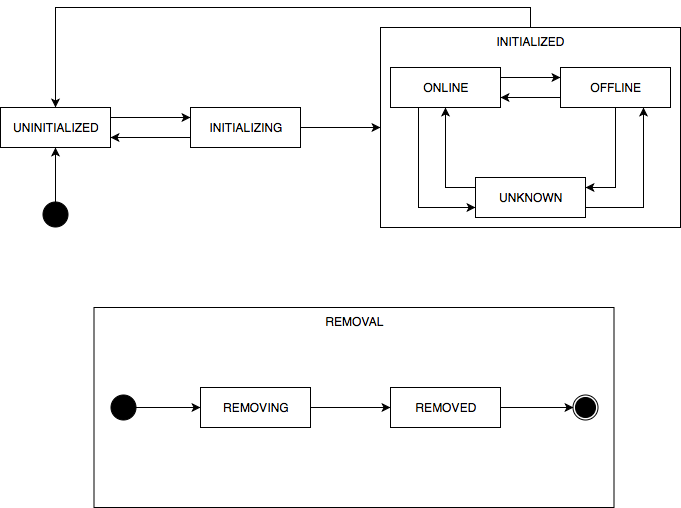
\includegraphics[width=1\textwidth]{images/Chapter_05/status-transtitions.png}
	\caption{Thing status transitions}
	\label{fig:status-transitions}
\end{figure}

The initial state of a Thing is UNINITIALIZED. From UNINITIALIZED the Thing goes into INITIALIZING. If the initialization fails, the 
Thing goes back to UNINITIALIZED. If the initialization succeeds, the binding sets the status of the Thing to UNKNOWN, ONLINE
or OFFLINE, which all mean that the Thing handler is fully initialized. From one of this states the Thing can go back into UNINITIALIZED,
REMOVING or REMOVED. The statuses REMOVING and REMOVED can also be reached from any of the other states.

\subsection{Items}
Eclipse SmartHome has a strict separation between the physical world (Things) and the application, which is built around the concept
of \textit{Items} (also known as the \textit{virtual layer}).

As mentioned at the beginning of this section, Items represent functionalities that can be used by the applications, mainly user 
interfaces or automation logic. Items also have a state and are used through events.

Each openHAB Item must be between the list of types that the table \ref{table:openhab-item-types} specifies.

\begin{table}[]
	\centering
	\resizebox{\textwidth}{!}{%
		\begin{tabular}{|l|l|l|}
			\hline
			\multicolumn{1}{|c|}{\textbf{Type}}                          & \multicolumn{1}{c|}{\textbf{Description}}                                                                          & \multicolumn{1}{c|}{\textbf{Command Types}}                                           \\ \hline
			Color                                                         & Color information (RGB)                                                                                            & \begin{tabular}[c]{@{}l@{}}OnOff, IncreaseDecrease,\\ Percent, HSB\end{tabular}       \\ \hline
			Contact                                                       & \begin{tabular}[c]{@{}l@{}}Item storing status of e.g. door/window \\ contacts\end{tabular}                        & OpenClose                                                                             \\ \hline
			DateTime                                                      & Stores date and time                                                                                               &                                                                                       \\ \hline
			Dimmer                                                        & \begin{tabular}[c]{@{}l@{}}Item carrying a percentage value for \\ dimmers\end{tabular}                            & \begin{tabular}[c]{@{}l@{}}OnOff, IncreaseDecrease,\\ Percent\end{tabular}            \\ \hline
			Group                                                         & \begin{tabular}[c]{@{}l@{}}Item to nest other Items / collect them \\ in Groups\end{tabular}                       &                                                                                       \\ \hline
			Image                                                         & Holds the binary data of an image                                                                                  &                                                                                       \\ \hline
			Location                                                      & Stores GPS coordinates                                                                                             & Point                                                                                 \\ \hline
			Number                                                        & \begin{tabular}[c]{@{}l@{}}Stores values in number format, takes \\ an optional dimension suffix\end{tabular}      & Decimal                                                                               \\ \hline
			\begin{tabular}[c]{@{}l@{}}Number\\ $<$dimension$>$\end{tabular} & \begin{tabular}[c]{@{}l@{}}Like Number, but with additional \\ dimension information for unit support\end{tabular} & Quantity                                                                              \\ \hline
			Player                                                        & \begin{tabular}[c]{@{}l@{}}Allows to control players (e.g. \\ audio players)\end{tabular}                          & \begin{tabular}[c]{@{}l@{}}PlayPause, NextPrevious, \\ RewindFastforward\end{tabular} \\ \hline
			Rollershutter                                                 & Typically used for blinds                                                                                          & \begin{tabular}[c]{@{}l@{}}UpDown, StopMove, \\ Percent\end{tabular}                  \\ \hline
			String                                                        & Stores texts                                                                                                       & String                                                                                \\ \hline
			Switch                                                        & Typically used for lights                                                                                          & OnOff                                                                                 \\ \hline
		\end{tabular}%
	}
	\caption{Types of Items in openHAB 2}
	\label{table:openhab-item-types}
\end{table}

\subsubsection{Group Items}
Group Items are a special kind of items that collect other Items into Groups. Group Items can themselves be members of other Group Items.
Depending on the user interface, it might display Group Items as single entries and provide navigation to its members.

With Group Items, it is also possible to derive their state from their member items. To derive a state the Group Item must be constructed using
a base Item and a Group function. Between the available Group functions we can find common operators such as EQUALITY, AND, OR, NAND,
NOR, SUM, AVG, MIN and MAX, among others.

\subsubsection{Links}
Links are the glue between Things and Items. They are associations between exactly one Thing Channel and one Item. If a Channel is 
linked to an Item, it is enabled, which means that the functionality that the Item represents is handled through the given Channel. 
Channels can be linked to multiple Items and Items can be linked to multiple Channels.

\subsection{Thing Discovery}
Thing Discovery is the process that the system makes in order to show the devices connected in your network. Many technologies, 
devices and systems can be discovered automatically or browsed through an API.

In Eclipse SmartHome bindings implement \textit{Discovery Services} for Things, which provide \textit{Discovery Results}. All Discovery 
Results are regarded as suggestions to the user and are put into the \textit{Inbox}.

\subsubsection{Inbox}
The Inbox holds a list of all discovered Things from all active discovery services. A discovery result represents a discovered Thing of a 
specific Thing type, that could be instantiated as a Thing. The result usually contains properties that identify the discovered Things 
further like IP address or a serial number. Each discovery result also has a timestamp when it was added to or updated in the Inbox 
and it may also contain a time to live, indicating the time after which it is be automatically removed from the Inbox.

Discovery results can either be ignored or approved, where in the latter case a Thing is created for them and they become available in 
the application. If an entry is ignored, it will be hidden in the Inbox without creating a Thing for it.

Eclipse SmartHome offers a service that is capable of automatically ignore discovery results on the Inbox, whenever a Thing is created
manually, that represents the same Thing, as the respective discovery result would create. This Thing would either have the same Thing
UID or the value of its representation property is equal to the representation property's value in the discovery result. The service is
enabled by default.

\subsection{Audio and Video}
Audio and voice features are an important aspect of any smart home solution as it is a very natural way to interact with the user.

Eclipse SmartHome comes with a very modular architecture that makes it possible in plenty of situations. At its core, there is the notion
of an \textit{audio stream}. Audio streams are provided by \textit{audio sources} and consumed by \textit{audio sinks}.

\begin{itemize}
	\item \textbf{Audio Streams} are essentially a byte stream with a given audio format.
	\item \textbf{Audio Formats} define the container (e.g. WAV), encoding, bit rate, sample frequency and depth and the bit order (little endian
	or big endian).
	\item \textbf{Audio Sources} are services capable of producing audio streams, which are able to support different formats and provide a
	stream in a requested format upon request. Typical audio sources are microphones, and a continuous stream is expected from them.
	\item \textbf{Audio Sinks} are services that accept audio streams of certain formats. Typically, these are expected to play the audio stream, 
	for example, a speaker.
	\item \textbf{Text-to-Speech (TTS)} services are similar to audio sources with respect to the ability to create audio streams. The different 
	is that they take a string as an input and will synthesize it to a spoken text using a given voice.
	\item \textbf{Speech-to-Text (STT)} services are similar to audio sinks, but they do not simply play back the stream, but convert it to a 
	plain string.
\end{itemize}

\begin{figure}
	\centering
	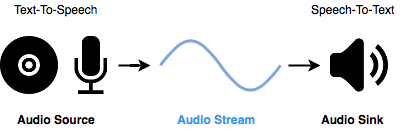
\includegraphics[width=0.7\textwidth]{images/Chapter_05/oh-audio-stream.png}
	\caption{Eclipse SmartHome audio stream scheme}
	\label{fig:oh-audio-stream}
\end{figure}

TTS and STT can provide information about the voices that they support, formats and locales. In TTS, each voice supports exactly one 
locale.

However, the STT service itself does not seem to be very useful. In order to process the generated string, there is the concept of a 
\textit{human language interpreter}.

\subsubsection{Human Language Interpreter}
A Human Language Interpreter takes a string as an input. It then derives actions from it, like sending commands to devices, or replies 
with a string, which opens the possibility to realize conversations. The figure \ref{fig:human-language-interpreter} shows a simple
schema of how it works.

In fact, an interpreter is not directly related to audio streams, but operates only with strings, so it is suitable either for voice 
assistants or chatbots for console, Twitter or other messaging services.

\begin{figure}
	\centering
	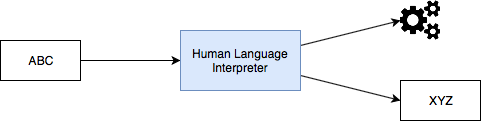
\includegraphics[width=0.9\textwidth]{images/Chapter_05/human-language-interpreter.png}
	\caption{A Human Language Interpreter transforms strings into other strings or commands}
	\label{fig:human-language-interpreter}
\end{figure}

Applications can dynamically choose which services to use, so that different sinks can be used for different use cases. Defaults can be 
set as configuration for all those services in case an application does not ask for any specific service.

\bigskip
\section{A Developer Perspective on openHAB}
OpenHAB 2 is a great open source, technology agnostic home automation platform that is able to manage lots of smart services and devices.

However, from a developer point of view, OpenHAB is not a complete platform itself, but rather an aggregation of features from different 
repositories, and mainly from Eclipse SmartHome:

\begin{itemize}
	\item \textbf{Eclipse SmartHome Framework}: the major parts of the core functionality are held by this repository. It contains bindings,
	services and items, amongst others, as openHAB does.
	\item \textbf{OpenHAB 2 Core and openHAB add-ons}: add-ons of openHAB that use the Eclipse SmartHome API.
	\item \textbf{Eclipse SmartHome Extensions}: openHAB is compatible with all extensions that are available for the Eclipse SmartHome 
	Framework and maintained within their repositories.
\end{itemize}

\subsection{Development environment set up}
Installing the development environment is a different process than installing OpenHAB itself, as a developer would require a local copy of
the source code of all elements, including the bindings, in an IDE. 

The process for installing OpenHAB 2 as a developer requires first to install Eclipse IDE with the OpenHAB-related repositories, which are 
the ones listed previously. It is usually required to have Maven 3 installed, and it is mandatory to have Oracle JDK 8 beforehand, because 
OpenHAB is fully coded in Java. \cite{openHABGithub}

The Eclipse installer downloads a copy of the repositories that the developer selects and installs and integrates them with Eclipse IDE 
automatically. Then, user can compile, run and debug the project from the IDE.

\begin{figure}
	\centering
	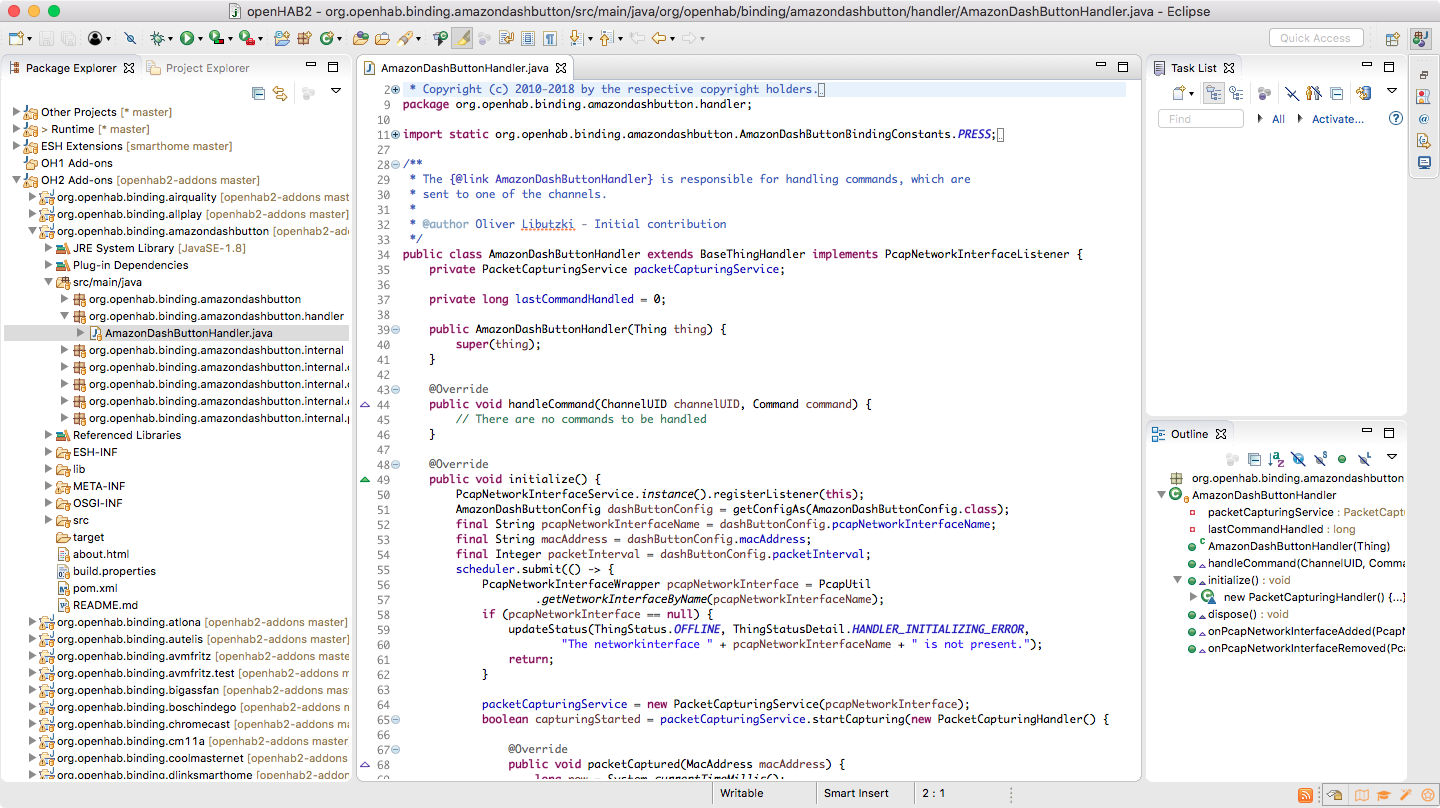
\includegraphics[width=1\textwidth]{images/Chapter_05/openhab2-ide.png}
	\caption{Eclipse SmartHome IDE with the OpenHAB repositories}
	\label{fig:openhab2-ide}
\end{figure}

\subsection{Platform structure}
Installing the platform as mentioned above provides us with a clear knowledge of the platform’s structure and makes it easy to perform 
any modification or addition to it. The OpenHAB 2 code is highly modular and presents a very well-defined organization, as can be seen 
in the figure \ref{fig:openhab2-structure}. Below there is a detailed explanation about the structure.

\begin{sidewaysfigure}
	\centering
	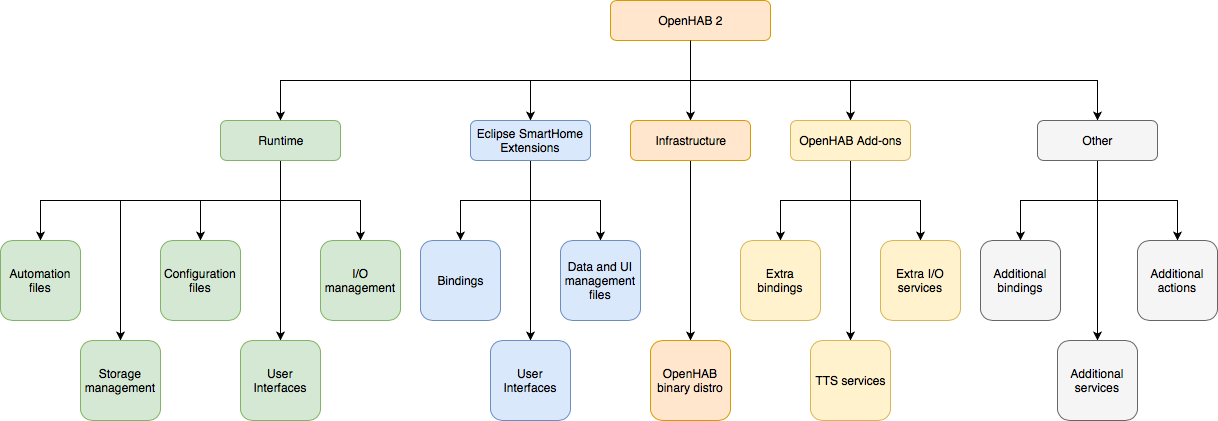
\includegraphics[width=1\textwidth]{images/Chapter_05/openhab2-structure.png}
	\caption{OpenHAB 2 structure}
	\label{fig:openhab2-structure}
\end{sidewaysfigure}

We can divide OpenHAB 2 in five parts, which are composed by one or more subsections that host differentiated code parts, each one
performing services, connecting to devices or managing the internal system:

\begin{itemize}
	\item \textbf{Runtime}: these are the basic libraries that OpenHAB need in order to execute properly, which come mostly from Eclipse 
	SmartHome. It is a big collection of different services:
	\begin{itemize}
		\item \textbf{Automation files}: they are in charge of the automated services in the platform, so they manage triggers and events.
		\item \textbf{Configuration files}: hosts the configuration files of the platform, such as the user folders or the listeners for the 
		item discovery process.
		\item \textbf{I/O management}: these libraries manage the inputs and outputs of the system, such as the MQTT communication 
		or the REST APIs.
		\item \textbf{Storage management}: a pair of libraries that are in charge of storing JSON files and managing MapDB databases. 
		\item \textbf{User interfaces}: the user interfaces OpenHAB provides by default are the BasicUI, the ClassicUI, the HomeBuilder 
		and the PaperUI (being this the most common in OpenHAB 2, as it requires zero manual configuration). These UIs are all part 
		of this repository and they come from OpenHAB, not from Eclipse SmartHome. However, Eclipse also provides packages for 
		internal aspects of the UI and for icons.
	\end{itemize}
	\item \textbf{Eclipse SmartHome Extensions}: functionality of Eclipse SmartHome can be extended through different additions, such 
	as bindings or other UIs. In this case, we can find:
	\begin{itemize}
		\item \textbf{Bindings}: they are the most important part of our system. Bindings integrate external systems, like services, protocols 
		or single devices to the platform. Therefore, the main purpose of a binding is to translate events from the Eclipse SmartHome 
		event bus to the external system and vice versa. This repository contains bindings for communicating via Bluetooth, or to Philips 
		Hue or DMX devices, amongst others. Many other bindings that OpenHAB support are located in the OpenHAB Add-ons repository.
		\item \textbf{User interfaces}: includes a bunch of UIs from Eclipse SmartHome, from which the OpenHAB UIs were created.
		\item \textbf{Data and UI management files}: this category contains additional configuration files and for managing UI’s elements.
	\end{itemize}
	\item \textbf{Infrastructure}: includes the binary files of OpenHAB. The end-user version of OpenHAB consists in only this repository.
	\item \textbf{OpenHAB add-ons}: these are libraries that OpenHAB introduced to Eclipse SmartHome. They extend its functionality to 
	make it a fully usable Home Automation environment.
	\begin{itemize}
		\item \textbf{Extra bindings}: OpenHAB created a huge number of new bindings for Eclipse SmartHome, from the binding for 
		Amazon Dash Button to the one for Samsung TVs. They cover an enormous range of smart devices, and the list is constantly growing.
		\item \textbf{Extra I/O services}: some bindings, like the Apple HomeKit binding, require I/O services that Eclipse SmartHome 
		does not originally include. In addition, new services like the OpenHAB cloud are also contained here.
		\item \textbf{TTS services}: OpenHAB 2 has added Text-To-Speech and Speech-To-Text functionality to Eclipse SmartHome, which is 
		also part of the OpenHAB add-ons repository.
	\end{itemize}
	\item \textbf{Other projects}: this repository holds libraries that are not part of any of the others, and it is a mix of additional bindings 
	(EnOcean, FritzBox…), additional actions and more services. Although they are located in this repository, they are officially supported 
	by OpenHAB.
\end{itemize}

\subsection{OSGi}
OpenHab is based on OSGi. The OSGi technology is a set of specifications that define a dynamic component system for Java. These 
specifications enable a development model where applications are dynamically composed of many different and reusable components. 

The OSGi specifications enable components to hide their implementations from other components while communicating through services, 
which are objects that are specifically shared between components.\cite{openHABDocs} The main features of OSGi are modularity, 
runtime dynamics and service orientation.

\subsubsection{OSGi Containers}
Different containers might implement different parts of the OSGi specifications and might provide slightly different API. The OpenHAB 
project uses Equinox, which is the reference implementation of the OSGi R4.x Core Specification and one of the mostly used as well.

Other popular open source OSGi containers are Apache Felix and Concierge. The container ProSyst OSGi Framework is widely used as 
well, but it is not free.

\subsubsection{Definitions}
\begin{itemize}
	\item \textbf{Bundle}: the OSGi components made by the developers. A bundle is comprised of Java classes and other resources, 
	which together can provide functions to end users.
	\item \textbf{Service}: any object that is registered in the OSGi Service Registry and can be looked up using its interface name(s).
	\item \textbf{Manifest}: descriptive information about the bundle, contained in its JAR file.
	\item \textbf{Service} Registry: enables a bundle to publish objects to a shared registry, advertised via a given set of Java interfaces.
\end{itemize}

\subsubsection{Layer Structure}
As the figure \ref{fig:osgi-layering} shows, the OSGi framework consists of layers build on top of each other:

\begin{itemize}
	\item \textbf{Module layer}: responsible for managing dependencies between bundles and for class loading.
	\item \textbf{Life Cycle Layer}: controls the life cycle of the bundles.
	\item \textbf{Service Layer}: defines a dynamic model of communication between different modules.
	\item \textbf{Actual Services}: this is the application layer, using all other layers.
	\item \textbf{Security Layer}: optional layer that manages permissions for different modules.
\end{itemize}

\begin{figure}
	\centering
	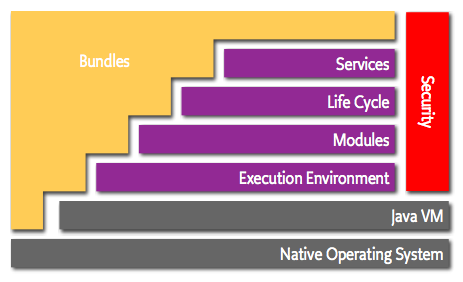
\includegraphics[width=0.8\textwidth]{images/Chapter_05/osgi-layering.png}
	\caption{OSGi layer structure}
	\label{fig:osgi-layering}
\end{figure}

\subsubsection{Bundles}
Bundles, also known as modules, are the smallest unit of modularization. Technically, they are a JAR file with additional meta information, 
which are stored in a file called \textit{manifest file}. The manifest file is part of the standard Java specification, but OSGi adds additional 
metadata to it in form of specific headers. The \textit{Bundle-SymbolicName} and the \textit{Bundle-Version} headers uniquely identify a 
bundle. In OSGi is allowed to have bundles with same name, but different version running at the same time.

The manifest contains information like the bundle dependencies. A bundle can depend on another bundle or on a package. Preferred way 
to define dependencies in a bundle is with \textit{Import-Package} and \textit{Export-Package} headers and not with \textit{Require-Bundle} 
header. This gives you an access only to the packages that you need and allows you to exchange the packages at a later point in time

The OSGi runtime uses the information about the dependencies to \textit{wire} the bundles and hides everything in this JAR unless it is 
explicitly exported. The dependencies to the Java standard libraries are managed by the \textit{Bundle-RequiredExecutionEnvironment} 
header, so it is not needed to import the Java core packages

Bundles are used often to register and consume services.

\subsubsection{Lifecycle}
OSGi is a dynamic platform. That means that bundles may be installed, uninstalled, started, stopped or updated at runtime, as the table
\ref{table:bundle-states-description} indicates. The OSGi specification defines a mechanism how to manage the dependencies between 
the bundles and the functionality that they provide. This is achieved with the help of the lifecycle concept.

The framework introduces a different states, transitions between these states and rules how this states are affecting the packages 
exported by the bundle and the services, that it provides. The table \ref{table:bundle-states-description} shows the possible states 
of an OSGi bundle with a short explanation

\begin{table}[]
	\centering
	\resizebox{\textwidth}{!}{%
		\begin{tabular}{|l|l|}
			\hline
			\multicolumn{1}{|c|}{\textbf{Status}} & \multicolumn{1}{c|}{\textbf{Description}}                                                                                                                                                                                                \\ \hline
			INSTALLED                             & \begin{tabular}[c]{@{}l@{}}The bundle has been installed into the OSGi container, but some of \\ it's dependencies are still not resolved. The bundle requires packages \\ that have not been exported by any other bundle.\end{tabular} \\ \hline
			RESOLVED                              & \begin{tabular}[c]{@{}l@{}}The bundle is installed and the all the dependencies at a class level \\ are resolved and wired. The bundle can export the packages, that it \\ provides.\end{tabular}                                        \\ \hline
			STARTING                              & \begin{tabular}[c]{@{}l@{}}A temporary state that the bundle goes through while the bundle is\\ starting, after all dependencies have been resolved. The bundle is \\ permitted to register services.\end{tabular}                       \\ \hline
			ACTIVE                                & The bundle is running                                                                                                                                                                                                                    \\ \hline
			STOPPING                              & \begin{tabular}[c]{@{}l@{}}A temporary state that the bundle goes through while the bundle \\ is stopping\end{tabular}                                                                                                                   \\ \hline
			UNINSTALLED                           & The bundle has been removed from the OSGi container                                                                                                                                                                                      \\ \hline
		\end{tabular}%
	}
	\caption{Bundle states description}
	\label{table:bundle-states-description}
\end{table}

The possible status transitions are shown in the state diagram in the figure \ref{fig:bundle-state-diagram}.

\begin{figure}
	\centering
	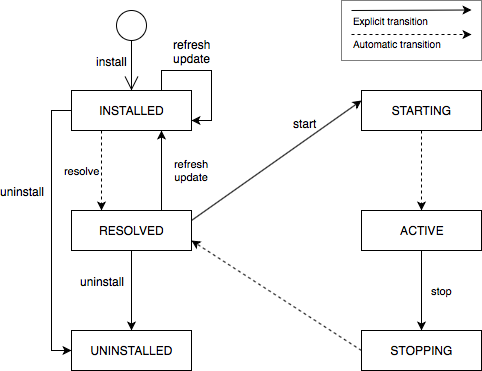
\includegraphics[width=0.8\textwidth]{images/Chapter_05/bundle-state-diagram.png}
	\caption{Bundle state diagram}
	\label{fig:bundle-state-diagram}
\end{figure}

\subsubsection{The Service Model}
The service model is another main concept that allows the bundles to communicate between each other.

In OSGi, a bundle can register a service in a central service registry under one or more service interface. Published services also 
have service properties associated with them in the registry. It is an important feature of OSGi, because it provides a central place
to register and get services. A bundle is permitted to register service objects at any time during the STARTING, ACTIVE or STOPPING 
states. Other bundles can go to the registry and list all objects, that are registered under a specific interface or class.

A bundle can therefore register a service, it can get a service and it can track for appearing and disappearing of service. Any 
number of bundles can register the same service type and any number of bundles can get the same service. The figure \ref{fig:osgi-services} 
represents a basic diagram of the service usage and tracking.

\begin{figure}
	\centering
	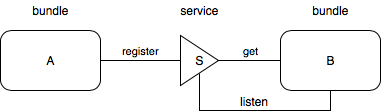
\includegraphics[width=0.7\textwidth]{images/Chapter_05/osgi-services.png}
	\caption{OSGi services \cite{osgiAlliance}}
	\label{fig:osgi-services}
\end{figure}

\subsubsection{Declarative Services}
In order to simplify the usage of services the OSGi Alliance has developed a model of managing services dynamically called Declarative 
Services. It is based on three main concepts:

\begin{itemize}
	\item \textbf{Declarative Services Container (DS)}: a module that is managing the lifecycle of a service component dynamically. 
	It activates and deactivated different components, basing its decisions on the information contained in the component description.
	\item \textbf{Service Component}: an object whose lifecycle is managed, usually by a component framework such as DS.
	\item \textbf{Component Description}: the declaration of a component, contained within an XML document in a bundle.
\end{itemize}

\paragraph{DS Container}
In order to use the Declarative Services, a bundle has to be started with an implementation of the DS container. In Equinox this 
bundle is called \textit{org.eclipse.equinox.ds}.

When a bundle that contains a component is added to the framework, DS reads its component description and if the conditions 
described in this file are fulfilled, the DS activates the component.

\paragraph{Components}
A component is a normal Java class, that can reference services and provide services. What makes it specific is that it is declared
in a XML file and is managed completely by the DS, so the DS instantiates the component, calls methods on it and manages its 
lifecycle.

A component in a bundle requires an XML description of the component, a \textit{Service-Component} manifest header, which locates 
the XML description, and an implementation class. There are three types of components: 
\begin{itemize}
	\item \textbf{immediate}: with \textit{immediate} attribute set to true
	\item \textbf{delayed}: with \textit{immediate} attribute set to false
	\item \textbf{factory}
\end{itemize}

A component goes through several states in his lifecycle:
\begin{itemize}
	\item \textbf{UNSATISFIED}: initial state of the Service Component, after the bundle is started.
	\item \textbf{REGISTERED}: temporary state, only \textit{delayed} components go through this state.
	\item \textbf{ACTIVE}: the component is active and component instance is created.
\end{itemize}

\begin{figure}
	\centering
	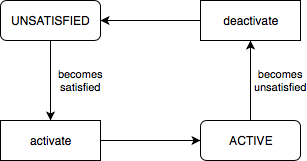
\includegraphics[width=0.6\textwidth]{images/Chapter_05/immediate-component-lifecycle.png}
	\caption{Immediate component lifecycle}
	\label{fig:immediate-component-lifecycle}
\end{figure}

\begin{figure}
	\centering
	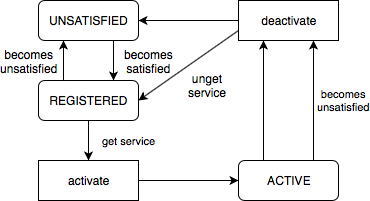
\includegraphics[width=0.6\textwidth]{images/Chapter_05/delayed-component-lifecycle.png}
	\caption{Delayed component lifecycle}
	\label{fig:delayed-component-lifecycle}
\end{figure}

The component lifecycle depends on the lifecycle of the bundle, that includes the component. Component must be enabled before it 
can be used. A component is enabled, when the component's bundle is started and disabled, when the bundle is stopped.

After the Component is enabled, it is moved to the UNSATISFIED state. The next step is to satisfy the component configuration.

The component configuration is satisfied when:
\begin{itemize}
	\item Component is enabled.
	\item All the component references are satisfied. A reference is satisfied when the reference specifies optional cardinality or 
	there is at least one target service for the reference. If the component has lazy initialization (the component is delayed), it is 
	moved to the REGISTERED state and it is waiting to be activated, when the service is requested (see figure 
	\ref{fig:delayed-component-lifecycle}).
	Otherwise (the component is immediate) as soon as its dependencies are satisfied, the component is activated (see figure
	\ref{fig:immediate-component-lifecycle}).
\end{itemize}

\bigskip
OpenHAB is much more than what I have explained in this chapter. But, as I will develop the project partially over openHAB,
I will explore more concepts from a developer perspective in the following chapter, like the installation of the system and the
configuration of its different parts.